%\let\negmedspace\undefined
%\let\negthickspace\undefined

\documentclass[journal,12pt,twocolumn]{IEEEtran}
\usepackage[cmex10]{amsmath}                            %Advanced Mathematics
\usepackage{setspace}
\usepackage{gensymb}                            %Deg/Cel/Ohm..
%\doublespacing
\DeclareMathSizes{10}{10.5}{7}{7}
\usepackage{polynom}                            %Polynomials
\singlespacing
%\usepackage{silence}
%Disable all warnings issued by latex starting with "You have..."
\usepackage{graphicx}
\usepackage{amssymb}                            %New symbols in math mode
%\usepackage{relsize}

%\usepackage{amsthm}
%\interdisplaylinepenalty=2500
%\savesymbol{iint}
%\usepackage{txfonts}
%\restoresymbol{TXF}{iint}
%\usepackage{wasysym}
\usepackage{amsthm}                             %Proof & Theorems
%\usepackage{pifont}
%\usepackage{iithtlc}
\usepackage{mathrsfs}
% \usepackage{txfonts}
\usepackage{stfloats}                           %Set, shrink and increase size
% \usepackage{steinmetz}
\usepackage{bm}                                 %Bold Greek letters
% \usepackage{cite}
% \usepackage{cases}
% \usepackage{subfig}
%\usepackage{xtab}
\usepackage{longtable}                          %Table through next page
%\usepackage{multirow}
%\usepackage{algorithm}
%\usepackage{algpseudocode}
\usepackage{enumitem}                           %Nested lists
\usepackage{mathtools}                          %Supplements ams-math
\usepackage{tikz}                               %Creates vector graphics
% \usepackage{circuitikz}
\usepackage{verbatim}
%\usepackage{tfrupee}
\usepackage[breaklinks=true]{hyperref}          %Manage links
%\usepackage{stmaryrd}
%\usepackage{tkz-euclide} % loads  TikZ and tkz-base
%\usetkzobj{all}
\usepackage{listings}                           %Inserts programming code
    \usepackage{color}                                            %%
    \usepackage{array}                                            %%
    \usepackage{longtable}                                        %%
    \usepackage{calc}                                             %%
    \usepackage{multirow}                                         %%
    \usepackage{hhline}                                           %%
    \usepackage{ifthen}                                           %%
  %optionally (for landscape tables embedded in another document): %%
    \usepackage{lscape}     
% \usepackage{multicol}
% \usepackage{chngcntr}
%\usepackage{enumerate}

%\usepackage{wasysym}
%\newcounter{MYtempeqncnt}
\DeclareMathOperator*{\Res}{Res}
\DeclareMathOperator*{\equals}{=}
%\renewcommand{\baselinestretch}{2}
\renewcommand\thesection{\arabic{section}}
\renewcommand\thesubsection{\thesection.\arabic{subsection}}
\renewcommand\thesubsubsection{\thesubsection.\arabic{subsubsection}}

\renewcommand\thesectiondis{\arabic{section}}
\renewcommand\thesubsectiondis{\thesectiondis.\arabic{subsection}}
\renewcommand\thesubsubsectiondis{\thesubsectiondis.\arabic{subsubsection}}

% correct bad hyphenation here
\hyphenation{op-tical net-works semi-conduc-tor}
\def\inputGnumericTable{}                                 %%

\lstset{
%language=C,
frame=single, 
breaklines=true,
columns=fullflexible
}
%\lstset{
%language=tex,
%frame=single, 
%breaklines=true
%}

\begin{document}

\newtheorem{theorem}{Theorem}[section]
\newtheorem*{problem}{Problem}
\newtheorem{proposition}{Proposition}[section]
\newtheorem{lemma}{Lemma}[section]
\newtheorem{corollary}[theorem]{Corollary}
\newtheorem{example}{Example}[section]

%\newtheorem{thm}{Theorem}[section] 
%\newtheorem{defn}[thm]{Definition}
%\newtheorem{algorithm}{Algorithm}[section]
%\newtheorem{cor}{Corollary}
\newcommand{\BEQA}{\begin{eqnarray}}
\newcommand{\EEQA}{\end{eqnarray}}
\newcommand{\define}{\stackrel{\triangle}{=}}
\newcommand*\circled[1]{\tikz[baseline=(char.base)]{
    \node[shape=circle,draw,inner sep=2pt] (char) {#1};}}
\bibliographystyle{IEEEtran}
\newcommand*{\permcomb}[4][0mu]{{{}^{#3}\mkern#1#2_{#4}}}
\newcommand*{\perm}[1][-3mu]{\permcomb[#1]{P}}
\newcommand*{\comb}[1][-1mu]{\permcomb[#1]{C}}
%\bibliographystyle{ieeetr}

\providecommand{\abs}[1]{\left\vert#1\right\vert}
\providecommand{\res}[1]{\Res\displaylimits_{#1}} 
\providecommand{\norm}[1]{\left\lVert#1\right\rVert}
\providecommand{\mbf}{\mathbf}
\providecommand{\pr}[1]{\ensuremath{\Pr\left(#1\right)}}
\providecommand{\qfunc}[1]{\ensuremath{Q\left(#1\right)}}
\providecommand{\sbrak}[1]{\ensuremath{{}\left[#1\right]}}
\providecommand{\lsbrak}[1]{\ensuremath{{}\left[#1\right.}}
\providecommand{\rsbrak}[1]{\ensuremath{{}\left.#1\right]}}
\providecommand{\brak}[1]{\ensuremath{\left(#1\right)}}
\providecommand{\lbrak}[1]{\ensuremath{\left(#1\right.}}
\providecommand{\rbrak}[1]{\ensuremath{\left.#1\right)}}
\providecommand{\cbrak}[1]{\ensuremath{\left\{#1\right\}}}
\providecommand{\lcbrak}[1]{\ensuremath{\left\{#1\right.}}
\providecommand{\rcbrak}[1]{\ensuremath{\left.#1\right\}}}
\theoremstyle{remark}
\newtheorem{rem}{Remark}
\newcommand{\sgn}{\mathop{\mathrm{sgn}}}


\providecommand{\res}[1]{\Res\displaylimits_{#1}} 

%\providecommand{\norm}[1]{\lVert#1\rVert}
\providecommand{\mtx}[1]{\mathbf{#1}}

\providecommand{\fourier}{\overset{\mathcal{F}}{ \rightleftharpoons}}
%\providecommand{\hilbert}{\overset{\mathcal{H}}{ \rightleftharpoons}}
\providecommand{\system}{\overset{\mathcal{H}}{ \longleftrightarrow}}
	%\newcommand{\solution}[2]{\textbf{Solution:}{#1}}
\newcommand{\solution}{\noindent \textbf{Solution: }}
\newcommand{\cosec}{\,\text{cosec}\,}
\providecommand{\dec}[2]{\ensuremath{\overset{#1}{\underset{#2}{\gtrless}}}}
\newcommand{\myvec}[1]{\ensuremath{\begin{pmatrix}#1\end{pmatrix}}}
\newcommand{\mydet}[1]{\ensuremath{\begin{vmatrix}#1\end{vmatrix}}}

%\numberwithin{equation}{subsection}
%\numberwithin{problem}{section}
%\numberwithin{definition}{section}
\makeatletter
\@addtoreset{figure}{problem}
\makeatother
\let\StandardTheFigure\thefigure
\let\vec\mathbf
%\renewcommand{\thefigure}{\theproblem.\arabic{figure}}
\renewcommand{\thefigure}{\theproblem}
%\setlist[enumerate,1]{before=\renewcommand\theequation{\theenumi.\arabic{equation}}
%\counterwithin{equation}{enumi}
%\renewcommand{\theequation}{\arabic{subsection}.\arabic{equation}}

%Title and Author
\title{ASSIGNMENT 3}
\author{CS21BTECH11053}

%\title{
%	\logo{Matrix Analysis through Octave}{\begin{center}\includegraphics[scale=.24]{tlc}\end{center}}{}{HAMDSP}
%}
% paper title
% can use linebreaks \\ within to get better formatting as desired
%\title{Matrix Analysis through Octave}
%
%
%author names and IEEE memberships
% note positions of commas and nonbreaking spaces ( ~ ) LaTeX will not break
% a structure at a ~ so this keeps an author's name from being broken across
% two lines.
% use \thanks{} to gain access to the first footnote area
% a separate \thanks must be used for each paragraph as LaTeX2e's \thanks
% was not built to handle multiple paragraphs
%
%\author{<-this % stops a space
%\thanks{}}
%}
% note the % following the last \IEEEmembership and also \thanks - 
% these prevent an unwanted space from occurring between the last author name
% and the end of the author line. i.e., if you had this:
% 
% \author{....lastname \thanks{...} \thanks{...} }
%                     ^------------^------------^----Do not want these spaces!
%
% a space would be appended to the last name and could cause every name on that
% line to be shifted left slightly. This is one of those "LaTeX things". For
% instance, "\textbf{A} \textbf{B}" will typeset as "A B" not "AB". To get
% "AB" then you have to do: "\textbf{A}\textbf{B}"
% \thanks is no different in this regard, so shield the last } of each \thanks
% that ends a line with a % and do not let a space in before the next \thanks.
% Spaces after \IEEEmembership other than the last one are OK (and needed) as
% you are supposed to have spaces between the names. For what it is worth,
% this is a minor point as most people would not even notice if the said evil
% space somehow managed to creep in.
%\WarningFilter{latex}{LaTeX Warning: You have requested, on input line 117, version}
% The paper headers
%\markboth{Journal of \LaTeX\ Class Files,~Vol.~6, No.~1, January~2007}%
%{Shell \MakeLowercase{\textit{et al.}}: Bare Demo of IEEEtran.cls for Journals}
% The only time the second header will appear is for the odd numbered pages
% after the title page when using the twoside option.
% 
% *** Note that you probably will NOT want to include the author's ***
% *** name in the headers of peer review papers.                   ***
% You can use \ifCLASSOPTIONpeerreview for conditional compilation here if
% you desire.
% If you want to put a publisher's ID mark on the page you can do it like
% this:
%\IEEEpubid{0000--0000/00\$00.00~\copyright~2007 IEEE}
% Remember, if you use this you must call \IEEEpubidadjcol in the second
% column for its text to clear the IEEEpubid mark.
% make the title area

\maketitle
\newpage
\bigskip
%\renewcommand{\thefigure}{\theenumi}
%\renewcommand{\thetable}{\theenumi}
%\renewcommand{\theequation}{\theenumi}
\begin{abstract}
  From NCERT Mathematics Class 11, Chapter 16 (Probability), Exercise 16.3
\end{abstract}
% IEEEtran.cls defaults to using nonbold math in the Abstract.
% This preserves the distinction between vectors and scalars. However,
% if the journal you are submitting to favors bold math in the abstract,
% then you can use LaTeX's standard command \boldmath at the very start
% of the abstract to achieve this. Many IEEE journals frown on math
% in the abstract anyway.
% Note that keywords are not normally used for peerreview papers.
%\begin{IEEEkeywords}
%Cooperative diversity, decode and forward, piecewise linear
%\end{IEEEkeywords}

% For peer review papers, you can put extra information on the cover
% page as needed:
% \ifCLASSOPTIONpeerreview
% \begin{center} \bfseries EDICS Category: 3-BBND \end{center}
% \fi
%
% For peer-review papers, this IEEEtran command inserts a page break and
% creates the second title. It will be ignored for other modes.
%\IEEEpeerreviewmaketitle



%Problem Declaration---------------------------------------
\begin{problem}[Ex:16.3, Question:2]
  %Problem---------------------------------------------------
  A coin is tossed twice, what is the probability that atleast one tail occurs? 
\end{problem}

%Solution--------------------------------------------------
\solution

%Random Variable-------------------------------------------
We will use binomial distribution here as we are repeating a Bernoulli trial with two possible outcomes \emph{Heads} or \emph{Tails}. We will consider getting \emph{Tails} as a success and \emph{Heads} as a failure. We will define random variable $X$ representing the number of successes. Given we have a total of $n = 2$ trials, $X \in \{0, 1, 2\}$.

Assuming a fair coin, the probability of success (gettings \emph{Tails}) in a single trial $p = 0.5$.

%Binomial Distribution-------------------------------------
The probability that $X = i$ is  given by
\begin{align}
  P(X = i) = \comb{n}{i} \times p^i \times (1-p)^{n-i}
  \label{eq:BinomProb}
\end{align}

%Cumulative Distribution-----------------------------------
One can define cumulative probability $P(X \leq i)$ as
\begin{align}
  P(X \leq i) = \sum_{r=i}^{n}\comb{n}{i} \times p^i \times q^{n-i}
  \label{eq:CumulProb}
\end{align}

%Answer------------------------------------------------------
Let us define another random variable $Y$ where $Y = 0$ when $X < 1$ and $Y = 1$ when $X \geq 1$. Random variable $Y$ represents a Bernoulli distribution. Hence
\begin{align}
  P(Y = 0) + P(Y = 1) = 1
  \label{eq:BernoulliY}
\end{align}
Note that
\begin{align}
  P(Y = 0) = P(X < 1) = P(X = 0)
  \label{eq:YrelX}
\end{align}
From
\eqref{eq:BinomProb}
and
\eqref{eq:YrelX}
\begin{align}
  P(Y = 0) = P(X = 0) = \comb{n}{0} \times p^0 \times (1-p)^n
  \label{eq:InterY}
\end{align}
Substituting $n = 2$ and $p = 0.5$ into
\eqref{eq:InterY}
\begin{align}
  &P(Y = 0) = \comb{2}{0}(0.5)^0(1-0.5)^2 = 0.25
  \label{eq:Yzero}
\end{align}
Using
\eqref{eq:YrelX}
and
\eqref{eq:Yzero}
\begin{align}
  P(Y = 1) = 1 - P(Y = 0) = 1 - 0.25 = \fbox{0.75}
  \label{eq:Final}
\end{align}

%Figure-----------------------------------------------------------
\underline{Graph}: The probability mass and cumulative distribution are plotted below.
\begin{figure}[!ht]
  \centering
  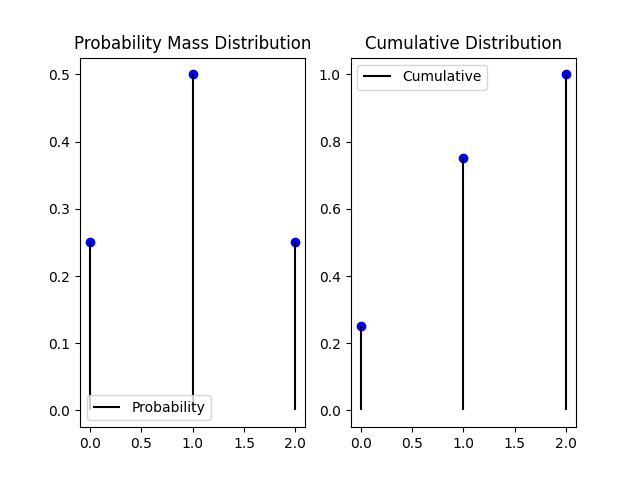
\includegraphics[width=\columnwidth]{../Figures/binom.png}
  \label{fig:Dis}
\end{figure}

\underline{Code Output}:
\begin{figure}[!ht]
  \centering
  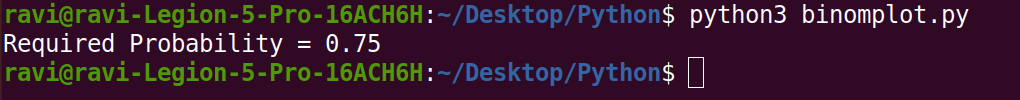
\includegraphics[width=\columnwidth]{../Figures/coin_output.png}
  \label{fig:Output}
\end{figure}

  
\end{document}
